\section{Autoencoders, Transformer}

Stiamo vedendo un esempio alla lavagna dove mostra come lavora un autoencoder e
che problema ha la struttura.

\textbf{La loss} è condizionata dai \textbf{vincoli di fattibilità} che ci sono. Nel senso,
si ha un valore in input \textbf{x} che si prende dai deti e lo si da in pasto all'\textbf{encoder}. Si ottiene uno
\textbf{spazio latente} che è un sottoinsieme dello spazio di input. Se prendiamo un punto nello spazio, però,
non siamo sicuri che possa \textbf{soddisfare} i vincoli che ci sono. La loss, allora, va aggiustata
tenendo conto di questo problema.

\[
    \mathcal{L}(x, \bar{x}) + \mathcal{L}_i(\bar{x})
\]

\begin{domanda}(Perché usare un autoencoder?)
    Voglio avere dei vettori che siano \textbf{rappresentativi} di quello che ho in input.
\end{domanda}

\textbf{Embedding:} Il risultato di applicare un \textbf{autoencoder} a qualcosa. Mappare \textbf{input} a \textbf{vettori}, applicando
il concetto di similarità per ottenere una semantica.

\textbf{Word Embedding}: Il risultato di costruire un latent space da un'insieme di parole.

Mappiamo le parole in \textbf{vettori}, ma non in modo generico. Vogliamo che
le parole che hanno un significato simile siano vicine nello spazio.
Probabilmente, questi punti vicini nello spazio \textbf{condividono} delle
feature tra loro. Parola chiave: \textbf{contesto} simile.

\[
    Embedding \implies Semantic
\]

\subsection{Cosa si può fare con gli autoencoder?}

Tutto ciò che si fa nel machine learning, può essere applicato a tutto quanto
con gli autoencoders.

\textbf{Feature Selection} è un problema molto generico per il \textit{machine learning}. Si ha un insieme di feature
e si vuole selezionare quelle più importanti. Come si applicano gli autoencoder in questo problema?

Qualcosa con \textbf{clustering}.

\textbf{Outlier detection | Anomaly detection}: In una distribuzione, un \textbf{outlier} è qualcosa che non rientra in questa distribuzione dei dati. Come outlier ci sono vari tipi
nel mondo reale:
\begin{itemize}
    \item Azioni strane
    \item Attacchi informatici
    \item Problemi di salute
    \item \dots
\end{itemize}

Ma la task difficile è effettivamente \textbf{come si definisce un outlier?}.
E' un concetto abbastanza complesso.

Immaginiamo di avere \textbf{3 cluster} con una nuvola di punti all'interno. Si
potrebbe calcolare una distanza dal centro e considerare i punti fuori dal
cluster come outlier. Gli autoencoder, però, risolvono questo problema in modo
più semplice.

Immaginiamio di avere $x_1, \dots, x_n$ dati. Si costruisce un autoencoder che
prende in input $x_i$ e si mappa $x_1 \rightarrow z_1, \dots, x_n \rightarrow
    z_n$. Si da in pasto al decoder e si ottiene $\bar{x_1}, \dots, \bar{x_n}$. Si
ha anche, quindi, un error $\varepsilon = ||x_i - \bar{x_i}||$. Questo errore
possiamo considerarlo come una \textbf{loss}. Maggiore sarà la loss, più
probabile è che il punto sia un outlier.

\textbf{Classification:} Consideriamo un dataset $x_1, \dots, x_n$ e alla fine vogliamo classificare con \textbf{yes} o \textbf{no} per una motivazione $m$ generica.
Si crea il latent space mappando $x_1 \rightarrow z_1, \dots, x_n \rightarrow z_n$ e si da il \textbf{latent space} in pasto ad una \textbf{feed forward network} che ritorna, appunto, \textbf{yes} o \textbf{no}.

Immaginiamo di avere delle immagini, tipo \textbf{gente che ha un cappello.}
Come facciamo a dire che le persone con il cappello siano vicine tra loro?
Magari ci saranno correlazione tra le feature, come ad esempio il colore degli
occhi, la pelle, i capelli, ecc...

Siccome il problema principale è che \textbf{non si ha controllo} su questo
problema, si utilizza un \textbf{variational autoencoder}. Lo scopo è quello di
condizionare \textbf{come vengono generati} i punti all'interno del latent
space. In pratica, \textbf{rendono lo spazio continuo}.

\[
    \mathcal{L}(x, \bar{x}) + \mathcal{L}_c(\bar{x}) + \mathcal{L}_s(E(x), FF(E(x)))
\]

dove con \textbf{E} si indica l'encoder e \textbf{FF} la feed forward network.

\textbf{Novità negli autoencoder}: Invece di costruire una funzione di loss da zero come abbiamo fatto sopra, si è cominciato ad usare un architettura diversa. L'architettura
non prende una singola unità per dataset, ma prende una \textbf{coppia} di elementi alla volta.

\begin{equation}
    \begin{aligned}
        x_1 \rightarrow E \rightarrow z_1 \rightarrow D \rightarrow \bar{x}_1 \\
        x_2 \rightarrow E \rightarrow z_2 \rightarrow D \rightarrow \bar{x}_2 \\
    \end{aligned}
\end{equation}

Alla fine qui si applica una loss diversa, calcolata in questo modo:

\[
    L(\pm d(z_1, z_2))
\]

dove $d$ è una funzione di distanza. Si vuole che la distanza tra i due punti
sia piccola se i due punti sono simili, mentre se sono diversi si vuole che sia
grande.

%grafico con 2 punti nelo spazio
\begin{figure}[H]
    \begin{center}
        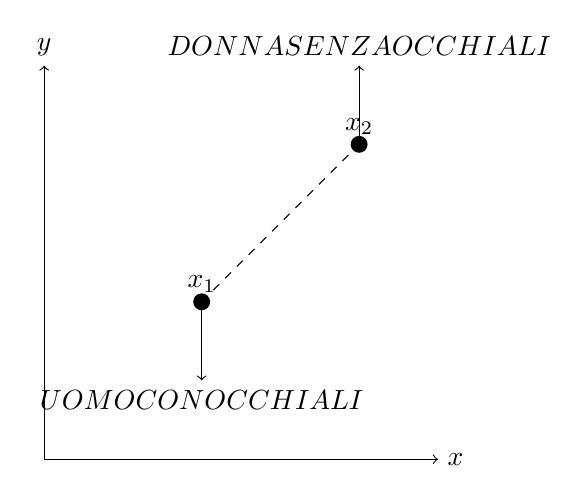
\begin{tikzpicture}
            \draw[->] (0,0) -- (5,0) node[right] {$x$};
            \draw[->] (0,0) -- (0,5) node[above] {$y$};
            \draw[fill=black] (2,2) circle (0.1) node[above] {$x_1$};
            \draw[fill=black] (4,4) circle (0.1) node[above] {$x_2$};

            %Scrivi UOMO su x1
            \draw[->] (2,2) -- (2,1) node[below] {$UOMO CON OCCHIALI$};

            %Scrivi DONNA SENZA OCCHIALI su x2 sopra
            \draw[->] (4,4) -- (4,5) node[above] {$DONNA SENZA OCCHIALI$};

            %retta che unisce i due punti
            \draw[dashed] (2,2) -- (4,4);
        \end{tikzpicture}
    \end{center}
    \caption{Esempio di spazio latente}
\end{figure}

Gli elementi che saranno sulla retta, circa, saranno elementi che avranno
feature di entrambi i punti, quindi ipoteticamente se stiamo parlando di
immagini, saranno uomini senza occhiali, donne con occhiali, ecc..., con altri
elementi che fanno parte di entrambi i punti.

\subsection{Accenno su Style Transfer}

Immaginiamo di avere 2 immagini:
\begin{itemize}
    \item Quadro
    \item Immagine normale
\end{itemize}

Diamo entrambe le immagini a 2 $Encoder$ e le uniamo in un unico $Encoder$. Si
ha un latent space e si ottiene una $Z$. \textbf{Non abbiamo un output} e va
calcolata una loss. La funzione è la seguente:
\[
    \mathcal{L}(Z, \alpha) + \mathcal{L}(Z, \beta)
\]

\subsection{Accenno su Stable Diffusion}

Assumiamo di avere un'immagine \textbf{corrotta} e sìvogliamo aggiungere
\textbf{noise random}, corrompendola. Noi sappiamo quali pixel sono quelli
corrotti.

L'architettura è \textbf{Encoder, Decoder}, la \textbf{loss} è ricostruire
\textbf{l'errore}. Vogliamo costruire \textbf{IL NOISE} che abbiamo aggiunto,
come risultato.

Si fanno degli step incrementali, aggiungendo man mano del noise all'immagine.
\textbf{Se si allena} un sistema con questa sequenza, cioè con l'immagine
chiara aggiungendo noise man mano, si \textbf{ottiene un risultato assurdo}: si
riesce a ricostruire l'immagine chiara.

\subsection{Autoencoder per le sequenze}

%immagine  dalla cartella
\begin{figure}[H]
    \centering
    \includegraphics[width=0.8\linewidth]{images/archRNN.png}
    \caption{Autoencoder per le sequenze}
    \label{fig:seq}
\end{figure}

Queste varie architetture si utilizzano per casi d'uso particolari:

\begin{itemize}
    \item One to One: Usata per le \textbf{classification}
    \item One to Many: Viene usata per \textbf{image captioning}
    \item Many to One: Usata per la sentiment analysis
    \item Many to Many: Usata per Machine Translation
    \item Many yo Many Synched: Video classification for each frame
\end{itemize}

\begin{domanda}(Nelle many to many dov'è il latent space?)

    Il latent space nel quarto esempio è il quadrato verde dal quale comincia la
    parte di deconding
\end{domanda}

\subsubsection{Seq2Seq}
Il modello si basa su un training che non da l'output di ogni time step al prossimo, ma sono il target dello step del training. A tempo di inferenza, il decoder
da l'output di ogni time step come input al prossimo.

\textit{Definizione di Chat:} Questo è un tipo di modello utilizzato per le sequenze, come le serie temporali o 
le sequenze di parole in un testo. Il modello è composto da due parti: un encoder, che trasforma l'input in una 
rappresentazione latente, e un decoder, che genera l'output a partire dalla rappresentazione latente. Durante 
l'addestramento, l'output di ogni passo temporale non viene dato come input al passo successivo. Invece, 
l'output di ogni passo temporale è il target per l'addestramento. Durante l'inferenza, l'output di ogni
 passo temporale viene dato come input al passo successivo.

\subsubsection{Training di Seq2Seq}


\begin{itemize}
    \item \textbf{Encoder}: \textit{word2id} + \textit{embedding}: Si passa ogni token della stringa fino ad un punto in cui si fa decoding.
    \item \textbf{Decoder}: Loop in cui tra tutte le parole si prende quella con la \textbf{probabilità maggiore}. \textit{Embedding} + \textit{id2word} 
\end{itemize}

\begin{figure}[H]
    \begin{center}
        \includegraphics[width=0.8\linewidth]{images/seq2seq.png}
    \end{center}
\end{figure}


\subsubsection{Problemi di questa architettura}

Il \textbf{contesto} della frase è tutto concentrato nel primo nodo dove si inizia il decoding. Serve il concetto di \textbf{attenzione}.
Proviamo a spiegarlo con un grafico:

%disegna 4 quadrati, ogni quadrato ha un testo sotto, ogni quadrato ha un quadrato sopra

Abbiamo una frase formato da delle parole. Abbiamo un inizio dove inizia il decoding. Per processare questo, l'attenzione è basata in base al nodo di \textbf{inizio}, si passa questo valore 
alla rete neurale, si usa una \textbf{softmax} calcolata dinamicamente ogni volta che va calcolata una nuova parola, basandosi sui pesi del contesto della parola da processare.


Tocca farsela spiegare da chat più tardi e mettere una cazzo di immagine porco dio.


\subsection{Da Seq2Seq ad accenni Transformer}

\textbf{Seq2Seq} è un modello che si basa su \textbf{RNN} e \textbf{LSTM}. Questi modelli hanno un problema: \textbf{sono lenti}. Per ogni parola, si deve aspettare che la rete neurale
faccia il suo lavoro. Non solo. Ciò che viene calcolato per le celle, rimane li. Non si può eliminare.

Il Paper \textit{Attention is All You Need} ha cambiato il mondo del NLP. Il modello si basa su \textbf{Transformer}. L'architettura ha le seguenti caratteristiche:
\begin{itemize}
    \item Nell'Encoding il testo è salvato in un vettore 
    \item Le parole sono processate con \textbf{Word Embedding}
    \item Il meccanismo di \textbf{attenzione} è il core di questa architettura
\end{itemize}

\begin{figure}[H]
    \begin{center}
        \includegraphics[width=0.8\linewidth]{images/transformer.png}
    \end{center}
    \caption{Architettura di Transformer}
\end{figure}

Spacchiamo l'input in pezzi:

\textbf{Input Embedding}: Si fa un embedding \textbf{parola per parola}.

Successivamente si ha un \textbf{positional encoding}: Ci serve mantenere l'informazione dell'\textit{ordine} delle parole. Per farlo, basta semplicemente 
avere una coppia (Indice, Parola Embeddata).

Si ha un \textbf{Multi-head Attention}: Serve per calcolare l'attenzione tra le parole. Si calcola l'attenzione tra le parole e si calcola la \textbf{query}.
Il valore viene passato ad una \textbf{Feed Forward Network}. Si ripete il processo, passando il risultato della \textbf{Feed Forward Network} alla \textbf{Multi-head Attention}, che 
successivamente ripassa il risultato alla \textbf{Feed Forward Network}, poi ad un \textbf{linear layer} e infine ad un \textbf{softmax}. Il risultato è un \textbf{vettore di probabilità}.

\textbf{Output Embedding}: E' il vettore delle frasi nella lingua da tradurre, anche questa con un positoinal encoding. Si passa questo ad una \textbf{masked multihead attention}, che vedremo poi come funziona, e che poi si collega alla \textbf{Multi-head attention} alla quale 
si era passata la prima \textbf{Feed Forward}.

Si utilizza questa struttura \textbf{shiftata a destra}; questo è il trick per sapere tutto l'input che si ha a disposizione della frase da tradurre e solamente la posizione della parola fino a quel punto.
per fare in modo che la rete possa farlo in un colpo solo, cioè il task per fare una predizione della frase di output in un colpo solo. 


Sommario: 
\begin{itemize}
    \item Input: la stringa
    \item Output: la stringa tradotta shiftata di uno a destra
    \item Se ho la frase: oggi sono qui, con posizione: 
    \begin{itemize}
        \item 0: oggi
        \item 1: sono
        \item 2: qui
    \end{itemize}
    \item Se mentre traduco sono alla posizione 2:
    \begin{itemize}
        \item 0: $\_$
        \item 1: oggi
        \item 2: sono
    \end{itemize}
    \item Ho la conoscenza fino alla posizione 2, e a runtime produco la stringa basandoci sulle probabilità che ho calcolato
\end{itemize}

\subsubsection{Cosa significa Masking?}

Come hanno fatto ad allenare CHAT-GPT? Quali sono stati gli \textbf{input, output}? Su cosa? A quali domande risponde? Come funziona? La risposta è nel \textbf{masking}.

Il concetto è quello di \textbf{aggiungere noise alle parole}, come in diffusion. ChatGPT ha imparato a rimuovere 
il noise dalle parole, ed è praticamente stato usato come un noise remover. In questo modo, la rete ha imparato.

\newpage
